
\subsection{{Description}}

    {In Problem Set 2, the ALU undergoes significant modifications in its core functionalities, tailored to specific operations outlined by the TA. Each modification serves a distinct purpose, altering the ALU core's behavior.}

    {The assigned functions for the ALU, derived from Problem 2 Table C, include:}

    \begin{itemize}
        \item   {{Producing the difference between A and B.}}
        \item   {{Generating the 2's complement of B.}}
        \item   {{Swapping the lower 4 bits of A with the lower 4 bits of B.}}
        \item   {{Producing null on the output.}}
        \item   {{Decrementing B by 5}}
        \item   {{Inverting the bit-significance order of A.}}
        \item   {{Shifting B to the left by three bits (SHL).}}
        \item   {{Incrementing A by 3.}}
        \item   {{Inverting all bits of B.}}
    \end{itemize}
    
    {This modification aligns with the lab's objectives, emphasizing VHDL syntax compatibility with Altera FPGA boards. ALU takes two 8-bit inputs (A and B) and a 16-bit input from the control unit, where the microcode serves as the operation-selector signal. Despite the 16-bit microcode, only nine distinct operations specified by the assigned functions are implemented in the modified ALU core.}
    
    {Upon implementation, the modified ALU executes the designated operation according to the assigned function, producing an 8-bit output referred to as "Result." This output is displayed on two 7-segment displays or LEDs, complying with the lab's visualization requirements. Similar to the initial ALU core design, ALU's purpose is to perform arithmetic and logical operations on inputs A and B based on the control unit's instruction.}
    
    {The modification introduces specific functionalities, enhancing the flexibility and capabilities of the ALU core within the broader GPU unit. Completing this problem set involves synthesizing, simulating, and verifying ALU's functionality, presenting the results, including waveforms, as part of the final report submission.}

    \subsubsection{{Inputs}}

        \begin{itemize}
            \item   {\textbf{A (8-bit)}: First input of 8 bits for arithmetic and logical operations.}
            \item   {\textbf{B (8-bit)}: Second 8-bit input for arithmetic and logical operations.}
            \item   {\textbf{Control Unit (16-bit)}: Microcode input from the control unit, functioning as the operation-selector signal.}
        \end{itemize}

    \subsubsection{{Outputs}}

        \begin{itemize}
            \item   {\textbf{Result (8-bit)}: Output representing the result of operations performed on inputs A and B.}
            \item   {\textbf{7-Segment Displays/LEDs}: Display output in hexadecimal format during FPGA board implementation.}
        \end{itemize}

    \subsubsection{{Purpose}}

        \begin{itemize}
            \item   {\textbf{A and B}: Serve as inputs for arithmetic and logical operations.}
            \item   {\textbf{Control Unit}: Determines the operation to be applied to inputs A and B.}
            \item   {\textbf{Result}: Represents the output of operations on A and B.}
            \item   {\textbf{7-Segment Displays/LEDs}: Display the output in hexadecimal format during FPGA board implementation.}
        \end{itemize}
    
    \subsubsection{{Timing Diagram}}

    \begin{figure}[H]
        \centering
        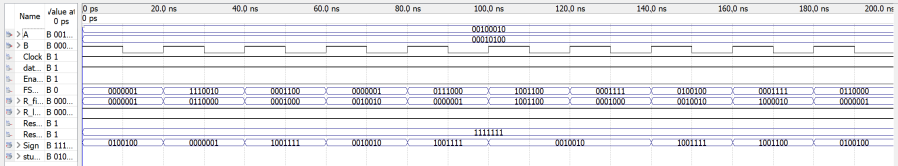
\includegraphics[width=15cm]{Pictures/ALU2WaveForm.png}
        \caption{{Timing Diagram of the Complete Logic Circuit 2}}
        \label{FSM}
    \end{figure}

    \subsubsection{{Block Diagram}}

        \begin{figure}[H]
            \centering
            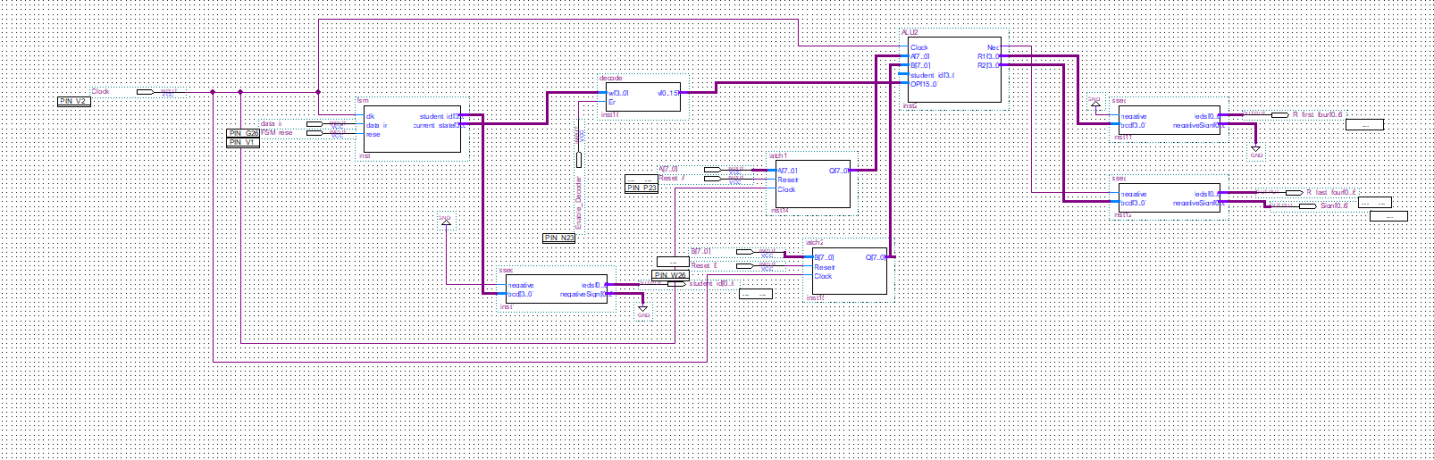
\includegraphics[width=15cm]{Pictures/P12BlockDia.png}
            \caption{{Block Diagram of the Complete Logic Circuit 2}}
            \label{FSM}
        \end{figure}


\subsection{{VHDL Code}}

    \subimport{./}{P2-VHDL}

